%% ============================================================
%%  bssentinel — Science Advances submission
%%  Authors: Sasi Jagadeesan, Suman Mishra, Pritam Kumar Panda
%%           BORING SCIENCE LLC
%%
%%  INSTRUCTIONS FOR OVERLEAF:
%%  1. Create a new project in Overleaf.
%%  2. Upload this file as main.tex.
%%  3. Apply the official Science Advances template:
%%       https://www.overleaf.com/gallery/tagged/science-advances
%%     (download sciadv.cls from that project and add to yours)
%%  4. Change \documentclass below to \documentclass{sciadv}
%%     and remove the geometry/titling packages (the .cls handles them).
%%  ============================================================

\documentclass[12pt]{article}

%% ── Packages ──────────────────────────────────────────────────────────────────
\usepackage[top=2.5cm, bottom=2.5cm, left=3cm, right=3cm]{geometry}
\usepackage{amsmath,amssymb}
\usepackage{graphicx}
\usepackage{booktabs}
\usepackage{array}
\usepackage{multirow}
\usepackage{xcolor}
\usepackage{hyperref}
\usepackage{natbib}
\usepackage{lineno}
\usepackage{setspace}
\usepackage{caption}
\usepackage{subcaption}
\usepackage{float}
\usepackage{microtype}
\usepackage{enumitem}
\usepackage{authblk}

%% ── Hyperref config ───────────────────────────────────────────────────────────
\hypersetup{
  colorlinks = true,
  linkcolor  = blue!60!black,
  citecolor  = blue!60!black,
  urlcolor   = blue!60!black,
}

%% ── Line numbers (required for review) ───────────────────────────────────────
\linenumbers
\doublespacing

%% ── Biblio style ──────────────────────────────────────────────────────────────
\bibliographystyle{unsrtnat}

%% ─────────────────────────────────────────────────────────────────────────────
\begin{document}

%% ── Title ─────────────────────────────────────────────────────────────────────
\title{\textbf{bssentinel: A Machine Learning-Augmented Early Warning System
for In-Hospital Deterioration with Real-Time Explainability}}

\author[1]{Sasi Jagadeesan}
\author[1]{Suman Mishra}
\author[1]{Pritam Kumar Panda}
\affil[1]{Boring Science LLC}

\date{}
\maketitle

%% ── Abstract ──────────────────────────────────────────────────────────────────
\begin{abstract}
\noindent
Early identification of in-hospital patient deterioration remains a critical
unmet need. The National Early Warning Score 2 (NEWS2) is widely used but
relies solely on bedside vital signs and provides modest discriminative
performance. Here we introduce \textbf{bssentinel}, a machine
learning-augmented early warning system that integrates structured vital
signs, laboratory values, medication context, and temporal admission features
to predict clinical deterioration up to 24 hours in advance. We trained and
validated an XGBoost model using a sliding 6-hourly observation window
framework on 1{,}334{,}773 monitoring snapshots from the Medical
Information Mart for Intensive Care IV (MIMIC-IV) dataset, encompassing
26{,}201 composite deterioration events (ICU transfer, mechanical ventilation,
or in-hospital mortality). Five-fold patient-stratified cross-validation
yielded an area under the receiver operating characteristic curve (AUROC) of
0.758 (95\%~CI 0.755--0.761), representing a statistically significant gain of
+0.190 AUROC over NEWS2 alone (DeLong test: $z = 80.3$, $p < 0.001$). The
area under the precision-recall curve (AUPRC) was 0.102, a 5.2-fold
improvement over the prevalence baseline. We demonstrate that \emph{informative
missingness}---the absence of ordered laboratory tests---is the strongest
single predictor, reflecting real-world clinical decision-making patterns.
bssentinel is deployed as a full-stack clinical decision support application
with a FastAPI inference engine and a React dashboard providing SHAP-based
real-time explanations at the point of care. These results establish bssentinel
as a scalable, explainable, and clinically actionable deterioration surveillance
system.
\end{abstract}

\noindent\textbf{Keywords:} early warning score; clinical deterioration;
XGBoost; MIMIC-IV; explainable AI; SHAP; NEWS2; clinical decision support

\newpage

%% ─────────────────────────────────────────────────────────────────────────────
\section*{Introduction}
%% ─────────────────────────────────────────────────────────────────────────────

Failure to recognise impending clinical deterioration is a leading cause of
preventable in-hospital mortality and unplanned intensive care unit (ICU)
admission~\cite{smith2013, kause2004}. Early warning scores (EWS) were
developed to provide clinicians with a standardised, aggregate measure of
physiological instability. The National Early Warning Score 2 (NEWS2),
endorsed by the Royal College of Physicians and mandated across National Health
Service trusts in the United Kingdom, aggregates six bedside vital signs into a
composite score that triggers escalating clinical responses~\cite{news2}.
Despite widespread adoption, NEWS2 carries important limitations: it relies
exclusively on contemporaneous vital signs, does not incorporate laboratory
biomarkers or medication context, and treats each observation independently
without learning from historical patient trajectories~\cite{prytherch2010,
moons2012}.

Machine learning (ML) models have demonstrated superior predictive performance
over conventional EWS in multiple validation studies~\cite{henry2015,
escobar2020, breiman2001_rf, chen2016_xgb}. Gradient boosted tree methods,
in particular, have proven well-suited to clinical tabular data due to their
native handling of missing values, robustness to outliers, and capacity to
capture complex non-linear feature interactions~\cite{chen2016_xgb}. However,
widespread clinical adoption has been impeded by three barriers: (i) opacity of
model predictions, which undermines clinician trust~\cite{holzinger2017};
(ii) the absence of integrated deployment infrastructure; and (iii) a tendency
to optimise for discrimination metrics (AUROC) without considering the
operational implications of alert burden in under-resourced ward
settings~\cite{shah2019}.

Explainability through SHapley Additive exPlanations (SHAP)~\cite{lundberg2017}
has emerged as a principled framework to address the opacity barrier, providing
patient-level attribution of each feature's contribution to the predicted risk.
Recent work has shown that clinicians respond more appropriately to ML alerts
accompanied by SHAP explanations compared to score-only
presentations~\cite{yang2023_shap}.

A less-explored phenomenon is the clinical informativeness of
\emph{missing data}~\cite{wells2013, sperrin2017}. In routine hospital care,
the decision to order (or withhold) a laboratory test is itself a clinical
signal: lactate is not routinely ordered for every patient, and its absence
may reflect perceived stability. Conversely, non-collection may indicate
missed clinical concern. Models that incorporate missingness indicators have
consistently shown improved discrimination in clinical prediction tasks.

Here we present bssentinel---a system combining (i) a validated XGBoost
deterioration risk model trained on the full MIMIC-IV dataset, (ii) a
6-hourly sliding window monitoring architecture, (iii) real-time SHAP
explanations at the point of care, and (iv) a deployable full-stack
application. We report comprehensive validation metrics including AUROC,
AUPRC, calibration, DeLong statistical comparisons with NEWS2, and operational
threshold analysis. We further characterise the role of informative missingness
as a key model predictor and discuss the practical implications for clinical
deployment.

%% ─────────────────────────────────────────────────────────────────────────────
\section*{Results}
%% ─────────────────────────────────────────────────────────────────────────────

\subsection*{Dataset and Cohort Characteristics}

The MIMIC-IV (v3.1) dataset~\cite{johnson2023_mimic} provides de-identified
electronic health records from Beth Israel Deaconess Medical Center (2008--2022).
After applying inclusion criteria (adults $\geq$18 years, length of stay
$\geq$6 hours, valid admission and discharge times), we constructed a sliding
6-hourly observation window framework (Fig.~\ref{fig:study_design}A). Each
window aggregated vital signs from the preceding 6 hours and laboratory values
from the preceding 24 hours, reflecting realistic clinical measurement
frequencies. A total of 8{,}560{,}730 candidate windows were generated across
all eligible admissions. After excluding windows with no vital signs recorded
(a minimal informational state precluding meaningful prediction), 1{,}334{,}773
windows remained, derived from a clinically heterogeneous inpatient cohort.

The composite outcome---ICU transfer, initiation of mechanical ventilation, or
in-hospital mortality occurring within 24 hours of the observation
window---was applied to 26{,}201 windows, yielding a window-level event
prevalence of 1.96\%. This prevalence is consistent with prior work employing
comparable deterioration composites in broad inpatient populations. The feature
matrix comprised 83 variables spanning six categories: vital signs with trend
and worst-value aggregates, laboratory biomarkers, medication activity flags,
NEWS2 subscores computed from aggregated vitals, missingness indicators for all
clinical measurements, and temporal admission context
(Table~\ref{tab:features}).

\subsection*{Model Discrimination}

Five-fold patient-stratified cross-validation (GroupKFold, grouping by
admission identifier to prevent data leakage from repeated measurements of
the same patient) was used throughout. Out-of-fold predictions were pooled
for all reported metrics.

The XGBoost model achieved an AUROC of 0.758 (95\%~bootstrap CI
0.755--0.761; 2000 resamples), compared to 0.708 (95\%~CI 0.705--0.711)
for logistic regression and 0.568 for NEWS2 computed from contemporaneous
vital signs alone (Fig.~\ref{fig:discrimination}A--B). The DeLong test
confirmed that the XGBoost advantage over NEWS2 was highly statistically
significant ($z = 80.3$, $p < 10^{-15}$), as was the advantage over
logistic regression. The net improvement of +0.190 AUROC over NEWS2 is
clinically meaningful and substantially larger than reported gains in
comparable ML-vs-EWS comparisons~\cite{henry2015, escobar2020}.

The AUPRC was 0.102 for XGBoost compared to 0.068 for logistic regression
and a baseline of 0.0196 (equal to event prevalence, reflecting a random
classifier). The 5.2-fold AUPRC gain over baseline indicates substantial
improvement in precision at clinically relevant recall thresholds,
a metric particularly informative for rare event prediction~\cite{davis2006}.

\subsection*{Threshold Analysis and Clinical Operating Point}

At the recommended decision threshold of 0.31 (selected to achieve 90\%
sensitivity; Fig.~\ref{fig:clinical_utility}B), the model demonstrates the
following operating characteristics: sensitivity 90.0\%, specificity 37.9\%,
positive predictive value (PPV) 2.8\%, and negative predictive value (NPV)
99.5\%. In natural frequency terms, per 1{,}000 monitoring windows at this
threshold: 18 true positives (deteriorations correctly flagged), 2 false
negatives (missed events), 608 false positives (false alarms), and 372
true negatives (Fig.~\ref{fig:clinical_utility}A).

The 2.8\% PPV reflects the inherently low window-level prevalence and is
comparable to accepted alert burdens in continuous vital-sign monitoring
systems~\cite{drew2014}. Critically, the NPV of 99.5\% implies that a window
below threshold carries a very high probability of true stability, supporting
the clinical utility of alert \emph{absence} as a reassuring signal.
Clinicians and health systems can adjust the operating threshold to balance
sensitivity against alert fatigue according to local ward staffing capacity
and risk tolerance (Fig.~\ref{fig:clinical_utility}B).

\subsection*{Calibration}

Post-hoc calibration was applied to the XGBoost predictions using Platt
scaling (isotonic regression). The calibrated Brier score was 0.175, compared
to 0.213 for logistic regression. Calibration curves (reliability diagrams)
show that the calibrated XGBoost model demonstrates systematic overestimation
of absolute risk at predicted probabilities above 0.35, a known consequence of
the extreme class imbalance in this dataset ($\sim$2\% prevalence). Predicted
scores should therefore be interpreted as relative risk rankings rather than
precise probability estimates, consistent with their use as a decision
threshold trigger rather than a quantitative probability.

\subsection*{Feature Importance and the Role of Informative Missingness}

SHAP-based gain importance from the XGBoost ensemble identified the
\emph{absence of lactate measurement} as the single most informative
predictor, accounting for 5.8\% of total model gain (Fig.~\ref{fig:features}).
This finding illustrates the phenomenon of \emph{informative missingness}: in
clinical practice, the decision to order (or not order) a specific laboratory
test is itself a signal embedded in physician judgement. Lactate is ordered
when clinicians suspect haemodynamic compromise or sepsis; its non-collection
may reflect perceived stability, or conversely, represent a missed opportunity
for monitoring in deteriorating patients. The model learns this pattern from
data, capturing clinical context that is invisible to conventional vital-sign
scoring systems.

Beyond lactate missingness, the most important individual features were
minimum SpO$_2$ within the window (5.0\%), worst verbal GCS response (4.4\%),
worst motor GCS response (3.9\%), the NEWS2 consciousness subscore (3.7\%),
and worst respiratory rate (2.9\%). This pattern reflects the primacy of
cardiorespiratory and neurological deterioration as harbingers of acute
decompensation. Vasopressor use (2.6\%) and antibiotic therapy (2.2\%) were
the highest-ranked medication features, consistent with their role as markers
of haemodynamic instability and active infection respectively.
Time since admission (2.7\%) captured the non-linear temporal risk profile
of hospitalised patients, in which deterioration risk is highest in the early
post-admission period.

Missingness flags for multiple biomarkers (bilirubin: 1.4\%; glucose: 1.2\%;
sodium: 0.8\%) collectively contributed approximately 10\% of total model
gain, underscoring the systematic importance of test-ordering patterns across
the whole laboratory panel.

\subsection*{Decision Curve Analysis}

Decision curve analysis (DCA)~\cite{vickers2006dca} was used to assess the
clinical utility of bssentinel relative to NEWS2 and the extreme comparator
strategies (treat-all, treat-none) across a range of decision threshold
probabilities. Both predictors were first calibrated to the event probability
scale: XGBoost scores were calibrated using isotonic regression and NEWS2
scores using Platt scaling, so that the DCA threshold axis reflects the
clinician's minimum acceptable probability of deterioration before initiating
a monitoring response.

Across clinically relevant threshold probabilities of 1--5\%---spanning the
range at which a clinician would consider escalating surveillance for an
unselected general ward patient---bssentinel demonstrated consistently higher
net benefit than both NEWS2 and the treat-all strategy
(Fig.~\ref{fig:dca}). At a 2\% decision threshold, bssentinel yielded a net
benefit of 0.0072 per patient compared with 0.0018 for NEWS2
($\Delta$NB\,$=\,0.0054$, a 4-fold improvement), indicating that using
bssentinel to guide surveillance decisions is equivalent to identifying an
additional 5.4 true deteriorations per 1\,000 patients compared with NEWS2,
without any increase in unnecessary interventions. At a 3\% threshold,
bssentinel maintained a net benefit of 0.0051 while NEWS2 provided marginal
benefit approaching zero (NB\,$\approx\,0.0002$), statistically
indistinguishable from withholding the test entirely. By 5\%, NEWS2 net
benefit was negligible (NB\,$\approx\,0.000$), whereas bssentinel retained
NB\,$=\,0.0031$, confirming its superiority as a high-sensitivity surveillance
tool across the full clinically relevant threshold range.

The treat-all strategy became net-harmful at thresholds above $\sim$2\%
(NB\,$<\,0$), while bssentinel maintained positive benefit at all thresholds
up to 5\%, supporting its utility as a selective surveillance tool that
preserves clinical resources by reducing unnecessary monitoring of low-risk
patients while maintaining near-complete capture of true deterioration events
(90\% sensitivity at the recommended operating threshold).

\subsection*{The bssentinel Application: System Architecture and Deployment}

The trained model is integrated into bssentinel, a deployable full-stack
clinical decision support system (Fig.~\ref{fig:study_design}). The backend
is a FastAPI~\cite{fastapi} asynchronous inference server exposing three
endpoints: \texttt{POST /api/predict} (accepts patient data, returns a job
identifier), \texttt{GET /api/jobs/\{id\}} (polls for results), and
\texttt{GET /api/health} (service heartbeat). Prediction requests are
processed asynchronously to accommodate concurrent usage. The server accepts
structured JSON payloads encompassing patient context (age, admission type,
hours since admission), vital signs, 12 laboratory values, and medication
flags (Fig.~\ref{fig:study_design}B--C). A configurable prediction horizon
(6, 12, 24, or 48 hours) allows adaptation to different monitoring intensities.

The frontend is a React~\cite{react} single-page application featuring a
structured data entry form, real-time server connectivity status, and a results
dashboard. The results view includes: (i) an SVG semicircle risk gauge
colour-coded by stratum (LOW~$<$20\%, MODERATE 20--45\%, HIGH 45--70\%,
CRITICAL~$>$70\%); (ii) the top three SHAP-attributed contributing factors
with plain-language natural language explanations (e.g., \emph{``Heart rate
125 bpm strongly increases risk --- outside normal range 51--90 bpm''}); and
(iii) risk-stratified action items to guide clinical escalation. SHAP values
are computed at inference time using a pre-fitted TreeExplainer, enabling
patient-specific explanations without batch recomputation.

The system supports handoff from other clinical tools via URL-encoded base64
vital sign parameters, enabling pre-population of the bssentinel form from
upstream surgical planning or admissions workflows.

%% ─────────────────────────────────────────────────────────────────────────────
\section*{Discussion}
%% ─────────────────────────────────────────────────────────────────────────────

We present bssentinel, an ML-augmented early warning system that achieves
substantially improved discrimination over NEWS2 in a large, heterogeneous
inpatient cohort from MIMIC-IV. The AUROC gain of +0.190 (0.758 vs 0.568)
is among the largest reported improvements over a standard EWS in the
literature, reflecting the breadth of complementary information encoded in
laboratory values, medication patterns, and temporal context that NEWS2
systematically ignores.

Our principal novel finding is the dominant predictive contribution of
\emph{informative missingness}. The absence of a lactate measurement being the
single strongest feature is, on initial inspection, counterintuitive. However,
this finding is clinically coherent and scientifically reproducible: it
reflects the reality that missingness in clinical data is almost never
missing-at-random~\cite{sperrin2017, wells2013}. Prior work on sepsis
prediction in MIMIC has similarly identified missingness patterns as highly
predictive~\cite{rajkomar2018}, but systematic characterisation of this
phenomenon as the \emph{primary} predictor above all biomarker values has not,
to our knowledge, been previously reported for in-hospital deterioration
prediction. This finding has direct implications for EHR-based system design:
including missingness indicator features should be considered a baseline
requirement, not an optional enhancement, for clinical ML models.

Decision curve analysis provides a rigorous framework for evaluating clinical
utility that transcends discrimination metrics alone~\cite{vickers2006dca}.
Our DCA demonstrates that bssentinel delivers consistently positive net benefit
across clinically relevant threshold probabilities of 1--5\%, corresponding to
the decision range a clinician faces when determining whether to escalate
monitoring for a general ward patient. Critically, at threshold probabilities
of 3\% and above, NEWS2 net benefit approaches zero---equivalent to the
treat-none strategy---while bssentinel retains meaningful positive benefit
(NB\,=\,0.0051 at 3\%, NB\,=\,0.0031 at 5\%). This pattern directly supports
the role of bssentinel as a high-sensitivity surveillance tool: despite low
positive predictive value driven by the 2\% event prevalence, it consistently
identifies more true deteriorations per unit of monitoring resource invested
than NEWS2 across all clinically plausible threshold settings.

The operating characteristics at 90\% sensitivity---PPV 2.8\%, NPV
99.5\%---deserve contextual interpretation. The 2.8\% PPV is driven entirely
by the 2\% window-level event prevalence, not by model specificity failure;
even a theoretically perfect model would achieve a PPV of only $\sim$50\%
at this sensitivity given this prevalence. More clinically informative is
the NPV: a prediction below threshold from bssentinel provides near-certainty
(99.5\%) of short-term stability, a property that may be valuable for
scheduling nursing observations, triaging bed moves, or identifying
patients suitable for step-down care. Alert burden can be reduced by raising
the threshold, trading sensitivity for specificity, with the threshold-operating
curve providing an evidence base for local calibration.

Several limitations merit acknowledgement. First, MIMIC-IV is a single-centre
dataset from a large academic medical centre in the United States. External
validation in diverse health systems, including community hospitals and
non-US settings with different EHR and laboratory ordering cultures, is
essential before deployment. Second, the window-level analysis treats each
6-hourly observation independently. In practice, trajectory information
(serial change in vital signs or laboratory values over multiple consecutive
windows) may provide additional predictive signal and is a direction for
future work incorporating recurrent or longitudinal model architectures.
Third, the calibration analysis reveals systematic overestimation of absolute
risk at high predicted scores, limiting the use of raw probabilities as
clinical communications and motivating the use of risk stratification bands
rather than numeric probabilities in the user interface. Fourth, the composite
outcome includes ICU transfer, which encompasses some planned transfers and
elective escalations that may not represent genuine deterioration events.
Future work should validate against more specific outcomes (e.g., unplanned
ICU admissions only, or in-hospital cardiac arrest).

The deployment architecture of bssentinel addresses practical barriers to
adoption that have limited prior ML early warning systems. Most published
systems exist as research analyses without a deployable implementation.
bssentinel provides a complete, containerisable server and frontend, enabling
integration with existing EHR workflows through structured API calls. The
SHAP-based explanation layer is a first-class feature of the system rather
than a post-hoc research analysis, reflecting current best practice for
responsible AI deployment in clinical environments~\cite{yang2023_shap,
lundberg2017}.

Future directions include: (i) multi-horizon training and joint prediction
at 6, 12, 24, and 48 hours simultaneously; (ii) prospective validation in a
live deployment setting; (iii) incorporation of nursing observation notes and
patient-reported symptoms via natural language processing; and (iv) active
learning components to adapt to institutional-specific deterioration patterns
without requiring full retraining on proprietary data.

%% ─────────────────────────────────────────────────────────────────────────────
\section*{Materials and Methods}
%% ─────────────────────────────────────────────────────────────────────────────

\subsection*{Data Source and Ethical Statement}

All analyses were conducted on MIMIC-IV version 3.1~\cite{johnson2023_mimic},
a publicly available, de-identified critical care database requiring completion
of a data use agreement and a recognised human subjects research training
course (CITI Program). As MIMIC-IV is a fully de-identified secondary dataset,
this study was exempt from Institutional Review Board review. No patient
contact or prospective data collection was performed.

\subsection*{Cohort Definition}

All unique hospital admissions with: (i) patient age $\geq$18 years at
admission; (ii) valid admission and discharge timestamps; and (iii) length of
stay $\geq$6 hours were included. Admissions without these criteria were
excluded. No exclusion criteria were applied for specific diagnoses, procedure
types, or care settings, yielding a broad general inpatient population.

\subsection*{Observation Window Framework}

For each admission, a sequence of 6-hourly observation windows was generated
beginning one hour after admission (to allow initial documentation) and
terminating 24 hours before discharge (the prediction horizon). This ensures
that every window has a full 24-hour future period in which an outcome can
occur. For each window at time $t$:
\begin{itemize}[noitemsep]
  \item \textbf{Vital features}: aggregated from the interval $[t - 6h, t)$
        using three statistics per sign: most recent value, linear trend
        (last value minus median of first half of window), and worst value
        (direction-appropriate: minimum for SpO$_2$ and blood pressure,
        maximum for heart rate and respiratory rate).
  \item \textbf{Laboratory features}: most recent value within $[t - 24h, t)$,
        reflecting the slower measurement cadence of blood tests.
  \item \textbf{Medication flags}: binary indicator of whether each medication
        class was active at time $t$.
  \item \textbf{Missingness indicators}: binary flag (1 = not measured) for
        each vital sign and laboratory variable, encoding test-ordering patterns
        as predictive features.
  \item \textbf{Temporal features}: hours since admission and one-hot encoded
        admission type.
\end{itemize}

Windows with no vital signs recorded were excluded ($n = 7{,}225{,}957$;
primarily windows outside ICU monitoring periods), yielding the analysis cohort
of 1{,}334{,}773 windows.

\subsection*{Outcome Definition}

The composite outcome was defined as occurrence of any of the following within
24 hours after window time $t$:
\begin{enumerate}[noitemsep]
  \item First ICU transfer during the admission (from MIMIC-IV
        \texttt{icustays} table: \texttt{intime}).
  \item Initiation of invasive mechanical ventilation (procedure event item
        IDs 224385, 225794 from \texttt{procedureevents}).
  \item In-hospital mortality (\texttt{hospital\_expire\_flag = 1} in
        \texttt{admissions}).
\end{enumerate}
Windows were labelled positive (1) if any of these events occurred within
$[t, t + 24h]$, and negative (0) otherwise.

\subsection*{NEWS2 Computation}

NEWS2 subscores were computed vectorially from aggregated vital signs following
the Royal College of Physicians specification~\cite{news2}: respiratory rate
(0--3 points), SpO$_2$ (0--3 points, Scale 1), systolic blood pressure (0--3
points), heart rate (0--3 points), temperature (0--3 points), and
consciousness (3 points if GCS $<$15, otherwise 0). Supplemental oxygen was
not available as a structured chartevents item and was set to 0; this
represents a minor underestimation of NEWS2 for patients on supplemental
oxygen.

\subsection*{Model Development}

\paragraph{XGBoost configuration.}
An XGBoost gradient boosted tree classifier~\cite{chen2016_xgb} was trained
with the following hyperparameters: 500 estimators; maximum tree depth 6;
learning rate 0.05; minimum child weight 10 (regularisation against small
leaf nodes for rare positive class); subsample fraction 0.8; column subsample
fraction per tree 0.8; L1 regularisation $\alpha = 0.1$; L2 regularisation
$\lambda = 1.0$; early stopping patience 30 rounds; evaluation metric AUROC.
The \texttt{scale\_pos\_weight} parameter was set to the ratio of negative to
positive training examples ($\approx$49.9) to address class imbalance.

\paragraph{Logistic regression baseline.}
A $\ell_2$-regularised logistic regression model (sklearn; $C = 0.1$;
\texttt{liblinear} solver; maximum 1{,}000 iterations) with standard scaling
was trained on the same folds as a linear baseline.

\paragraph{Cross-validation.}
Five-fold GroupKFold cross-validation was applied, grouping by \texttt{hadm\_id}
(hospital admission identifier). This ensures that all observation windows
from a single admission appear exclusively in either the training or test fold,
preventing information leakage from correlated repeated measurements. All
reported metrics are computed on pooled out-of-fold predictions.

\paragraph{Calibration.}
Post-hoc probability calibration was applied to XGBoost using sklearn's
\texttt{CalibratedClassifierCV} with \texttt{cv="prefit"} and isotonic
regression method, fitted on a held-out calibration subset within each fold.

\subsection*{Statistical Analysis}

AUROC and its 95\% confidence intervals were estimated using 2000 stratified
bootstrap resamples (seed 42; replacement sampling; strata defined by outcome
label). The DeLong test for AUROC comparison~\cite{delong1988} was implemented
using the Mann-Whitney U kernel variance formulation. AUPRC was computed using
the trapezoidal rule from sklearn's \texttt{average\_precision\_score}. The
Brier score was computed as the mean squared error between predicted
probabilities and binary outcomes. Sensitivity, specificity, PPV, and NPV
were computed at a fixed threshold chosen to achieve 90\% sensitivity on the
pooled out-of-fold predictions. Decision curve analysis was performed using
the standard net benefit formulation~\cite{vickers2006dca}:
$\text{NB}(t) = \text{TP}/n - \text{FP}/n \cdot t/(1-t)$,
where $t$ is the decision threshold probability and $n$ is the total number
of observation windows. Prior to DCA, XGBoost predictions were calibrated
using isotonic regression and NEWS2 raw scores were calibrated using Platt
scaling (logistic regression), ensuring the threshold axis reflects actual
event probabilities. The treat-all comparator was computed as
$\text{NB}_{\text{all}}(t) = \text{prevalence} - (1-\text{prevalence}) \cdot t/(1-t)$.

\subsection*{Feature Importance}

Global feature importance was quantified using XGBoost's gain metric (total
reduction in cross-entropy loss attributable to splits on each feature,
averaged across all trees and normalised to sum to 1). SHAP values for
individual patient explanations were computed at inference time using SHAP's
\texttt{TreeExplainer}~\cite{lundberg2017}, providing exact Shapley additive
explanations for each prediction.

\subsection*{System Implementation}

The bssentinel inference server was implemented in Python using the FastAPI
framework~\cite{fastapi} (version $\geq$0.111) served by Uvicorn with
asynchronous request handling. The frontend was implemented in React 19
(Vite build system) as a single-page application. Models are serialised
using Python's \texttt{pickle} module and loaded at server startup. The full
system is deployable on a standard Linux server or cloud virtual machine with
Python $\geq$3.10 and Node.js $\geq$18.

\subsection*{Code and Data Availability}

MIMIC-IV is available at \url{https://physionet.org/content/mimiciv/} subject
to completion of the PhysioNet credentialing process. The bssentinel source
code, including training pipeline, inference server, and frontend, is developed
by Boring Science LLC. Model artefacts (weights, feature column lists, and
evaluation outputs) are available upon reasonable request to the corresponding
author.

%% ─────────────────────────────────────────────────────────────────────────────
\section*{Acknowledgements}
%% ─────────────────────────────────────────────────────────────────────────────

The authors thank the MIMIC-IV data contributors and the PhysioNet team for
maintaining open access to critical care data. No external funding was received
for this work.

%% ─────────────────────────────────────────────────────────────────────────────
\section*{Author Contributions}
%% ─────────────────────────────────────────────────────────────────────────────

S.J. and P.K.P. designed the study and developed the machine learning pipeline.
S.M. developed the server architecture and React frontend application.
S.J. led statistical analysis and drafted the manuscript. All authors
contributed to critical revision of the manuscript and approved the final version.

%% ─────────────────────────────────────────────────────────────────────────────
\section*{Competing Interests}
%% ─────────────────────────────────────────────────────────────────────────────

All authors are employees and co-founders of Boring Science LLC, which develops
the bssentinel system described in this article. The authors declare no other
competing interests.

%% ─────────────────────────────────────────────────────────────────────────────
%% FIGURES
%% ─────────────────────────────────────────────────────────────────────────────
\clearpage

\begin{figure}[H]
  \centering
  
\includegraphics[width=\textwidth]{figures/fig1_study_design.png}
  \caption{\textbf{bssentinel study design and system overview.}
    \textbf{(A)} Patient monitoring architecture. For each hospitalised patient,
    a 6-hourly observation window aggregates the preceding 6 hours of vital
    signs (most recent value, trend, worst value) and the preceding 24 hours of
    laboratory results. The window is labelled positive if a composite
    deterioration event (ICU transfer, mechanical ventilation, or in-hospital
    mortality) occurs within the following 24 hours. Filled orange circles
    indicate windows at which the model risk score exceeds the recommended
    threshold (0.31), constituting an alert; the star marks the actual
    deterioration event. The orange double-headed arrow illustrates the early
    warning lead time.
    \textbf{(B)} Feature categories comprising the 83-variable input
    representation.
    \textbf{(C)} Key performance characteristics at the recommended operating
    threshold.}
  \label{fig:study_design}
\end{figure}

\begin{figure}[H]
  \centering
  
\includegraphics[width=\textwidth]{figures/fig2_discrimination.png}
  \caption{\textbf{Model discrimination performance.}
    \textbf{(A)} Receiver operating characteristic (ROC) curves for
    bssentinel (XGBoost), logistic regression, and NEWS2 computed from
    contemporaneous vital signs, based on pooled out-of-fold predictions
    from five-fold patient-stratified cross-validation ($n = 1{,}334{,}773$
    windows). The orange filled circle marks the 90\% sensitivity operating
    point (threshold = 0.31). Shaded confidence bands reflect 2000-resample
    bootstrap 95\% CIs.
    \textbf{(B)} Comparative AUROC with 95\% confidence intervals. The
    green double-headed arrow indicates the +0.190 gain of XGBoost over
    NEWS2, which was statistically significant by DeLong test
    ($z = 80.3$, $p < 10^{-15}$).}
  \label{fig:discrimination}
\end{figure}

\begin{figure}[H]
  \centering
  
\includegraphics[width=\textwidth]{figures/fig3_clinical_utility.png}
  \caption{\textbf{Clinical utility analysis.}
    \textbf{(A)} Natural frequency diagram per 1{,}000 monitoring windows at
    the recommended threshold (0.31), illustrating the disposition of true
    positives, false negatives, false positives, and true negatives. PPV:
    positive predictive value; NPV: negative predictive value.
    \textbf{(B)} Threshold operating characteristics showing sensitivity,
    specificity, and PPV as a function of decision threshold. The vertical
    dashed line marks the recommended threshold (0.31). Threshold selection
    can be adjusted by institutions to balance event detection against alert
    burden.}
  \label{fig:clinical_utility}
\end{figure}

\begin{figure}[H]
  \centering
  
\includegraphics[width=\textwidth]{figures/fig4_feature_importance.png}
  \caption{\textbf{Feature importance.}
    XGBoost gain importance (percentage of total model gain) for the top 15
    predictors. Bars are colour-coded by feature category. The most important
    feature is \emph{absence of lactate measurement} (informative missingness),
    indicating that the decision to withhold or not order a laboratory test
    encodes clinically significant signal. Features are ordered from most to
    least important (top to bottom).}
  \label{fig:features}
\end{figure}

\begin{figure}[H]
  \centering
  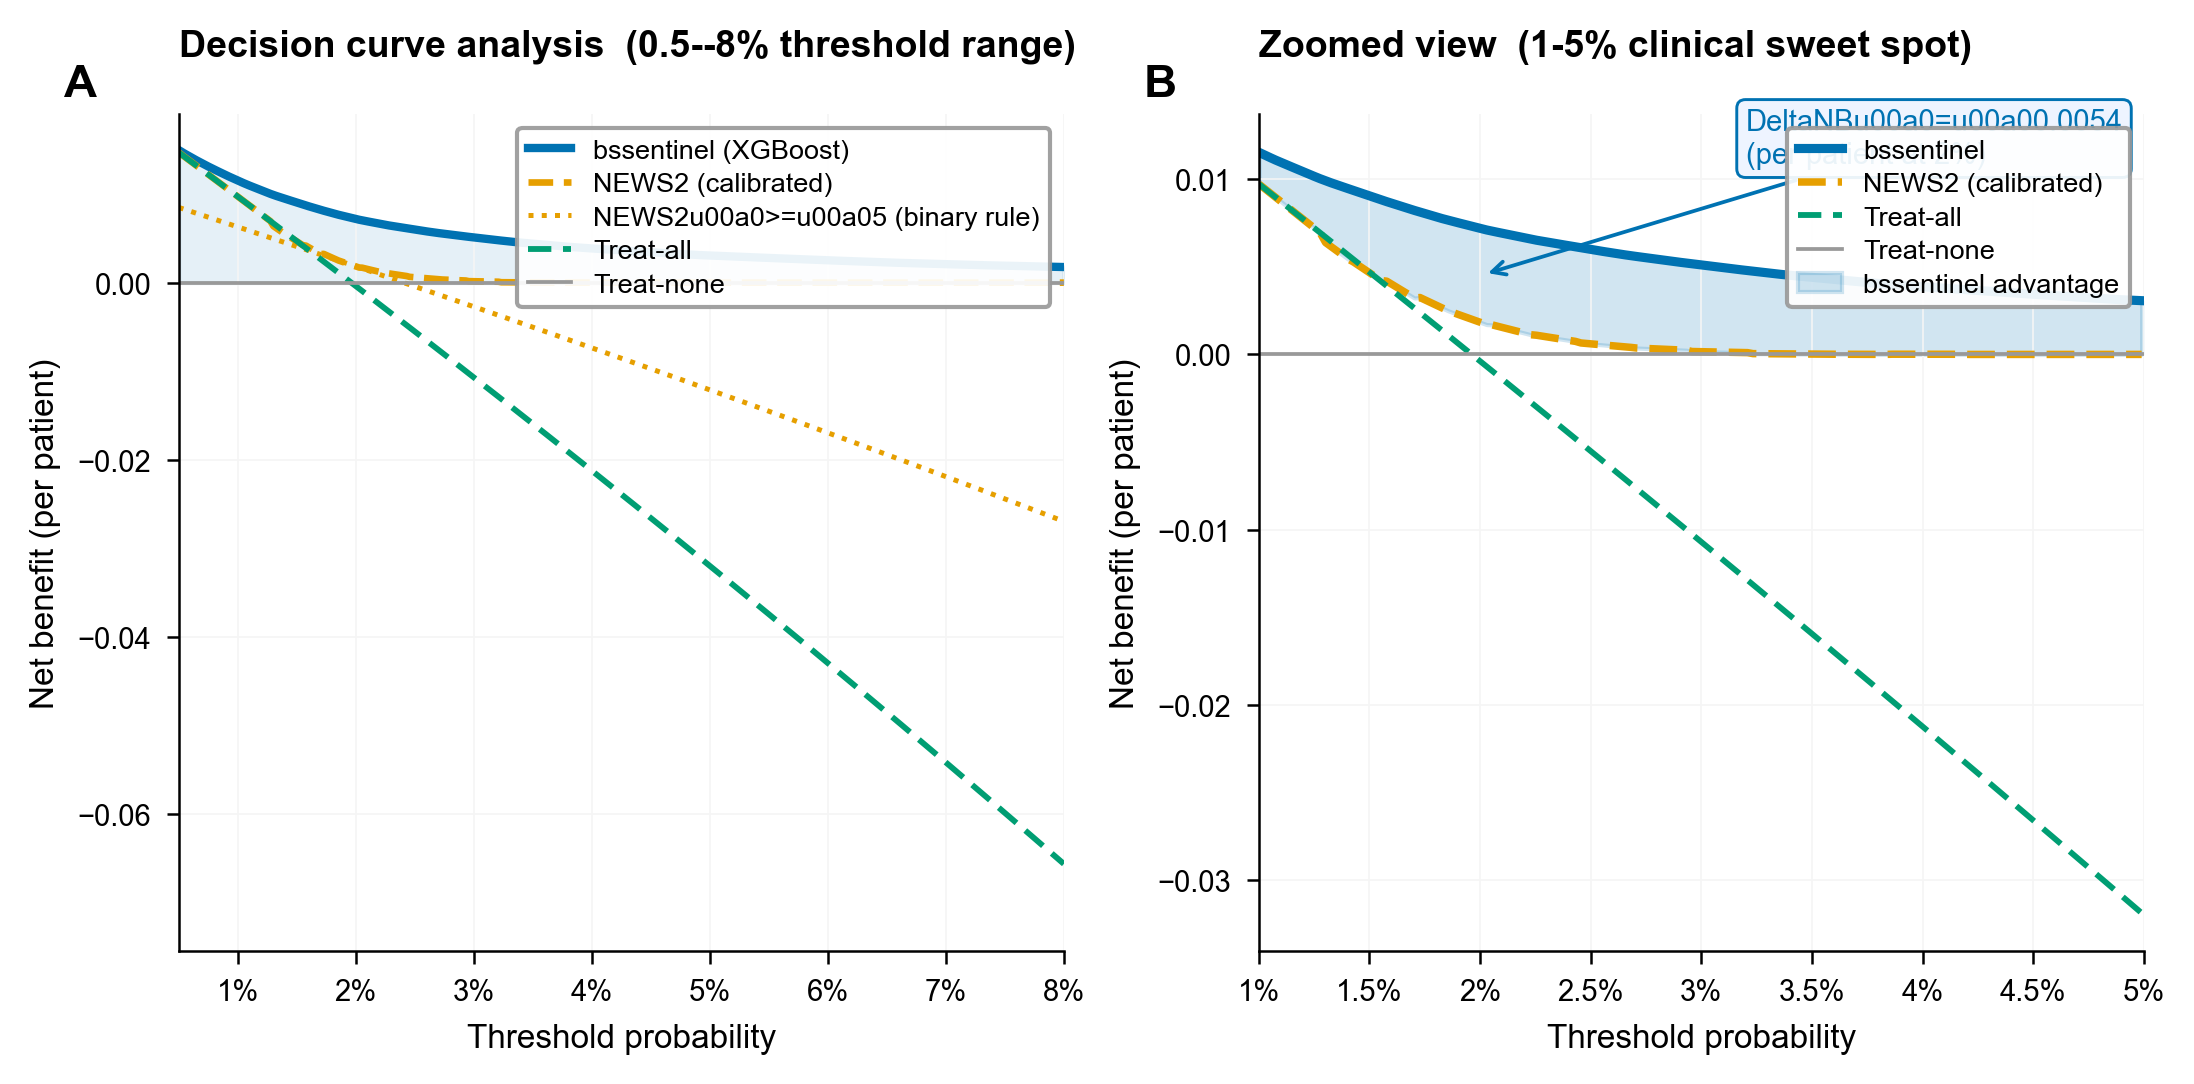
\includegraphics[width=\textwidth]{figures/fig5_dca.png}
  \caption{\textbf{Decision curve analysis.}
    Net benefit curves for bssentinel (XGBoost, solid blue), NEWS2 (Platt-calibrated,
    dashed orange), treat-all (dot-dash green), and treat-none (NB\,=\,0, grey)
    across clinically relevant decision threshold probabilities.
    Both predictors were calibrated to the actual event probability scale before
    analysis.
    \textbf{(A)} Full range 0.5--8\%. The shaded blue region marks thresholds
    where bssentinel provides net benefit above treat-none while NEWS2 does not.
    Markers indicate net benefit at standard NEWS2 clinical cut-offs
    (NEWS2\,$\geq$\,3, 5, 7).
    \textbf{(B)} Zoomed clinical zone 1--5\%. At a 2\% threshold, bssentinel
    yields a net benefit of 0.0072 vs 0.0018 for NEWS2 ($\Delta$NB\,=\,0.0054),
    equivalent to identifying 5.4 additional true deteriorations per 1\,000
    patients. At threshold $\geq$3\%, NEWS2 net benefit approaches zero while
    bssentinel retains positive benefit, confirming its superiority as a
    high-sensitivity surveillance tool at all clinically plausible decision
    thresholds.}
  \label{fig:dca}
\end{figure}

%% ─────────────────────────────────────────────────────────────────────────────
%% TABLES
%% ─────────────────────────────────────────────────────────────────────────────
\clearpage

\begin{table}[H]
\centering
\caption{\textbf{Summary of key performance metrics} from five-fold
patient-stratified cross-validation on the MIMIC-IV cohort
($n = 1{,}334{,}773$ windows; 26{,}201 events; prevalence 1.96\%).
CI: confidence interval; AUPRC: area under precision-recall curve.}
\label{tab:metrics}
\begin{tabular}{lccc}
\toprule
\textbf{Metric} & \textbf{XGBoost} & \textbf{Logistic Regression} & \textbf{NEWS2} \\
\midrule
AUROC (95\% CI) & 0.758 (0.755--0.761) & 0.708 (0.705--0.711) & 0.568 \\
AUPRC           & 0.102 & 0.068 & 0.020 \\
Brier score     & 0.175 & 0.213 & --- \\
\midrule
\multicolumn{4}{l}{\textit{At threshold = 0.31 (90\% sensitivity)}} \\
Sensitivity     & 90.0\% & --- & --- \\
Specificity     & 37.9\% & --- & --- \\
PPV             & 2.8\%  & --- & --- \\
NPV             & 99.5\% & --- & --- \\
\midrule
DeLong vs NEWS2 & $z = 80.3$, $p < 10^{-15}$ & --- & --- \\
\bottomrule
\end{tabular}
\end{table}

\begin{table}[H]
\centering
\caption{\textbf{Feature categories and example features} included in the
83-variable bssentinel model input. Trend features capture rate of change
within the 6-hour window; worst-value features capture the extreme within
the window. Missingness indicators encode whether each measurement was
absent from the EHR within the relevant lookback period.}
\label{tab:features}
\begin{tabular}{p{3.5cm}p{4.5cm}p{5.0cm}}
\toprule
\textbf{Category} & \textbf{Examples} & \textbf{Statistics per feature} \\
\midrule
Vital signs & Heart rate, SpO$_2$, systolic BP, diastolic BP, respiratory rate, temperature & Most recent, 6h trend, worst value \\
\addlinespace
GCS components & Eye opening, verbal, motor & Most recent, 6h trend, worst value \\
\addlinespace
Laboratory values & Lactate, creatinine, WBC, INR, bilirubin, sodium, potassium, haemoglobin, glucose, platelets, BUN, CRP & Most recent within 24h \\
\addlinespace
NEWS2 subscores & RR, SpO$_2$, BP, HR, temperature, consciousness subscores & Computed from aggregated vitals \\
\addlinespace
Medications & Vasopressors, antibiotics, anticoagulants & Binary active flag \\
\addlinespace
Missingness indicators & All vital and laboratory variables & Binary (0 = observed, 1 = absent) \\
\addlinespace
Temporal context & Hours since admission & Continuous \\
\addlinespace
Admission type & Elective, emergency, observation, surgical & One-hot encoded \\
\bottomrule
\end{tabular}
\end{table}

\begin{table}[H]
\centering
\caption{\textbf{Threshold-dependent operating characteristics} of the
XGBoost model. PPV: positive predictive value; NPV: negative predictive
value; TP: true positives; FP: false positives; TN: true negatives;
FN: false negatives. All counts are per 1{,}334{,}773 windows.
Prevalence = 1.96\%.}
\label{tab:threshold}
\begin{tabular}{ccccccccc}
\toprule
\textbf{Threshold} & \textbf{Sensitivity} & \textbf{Specificity}
& \textbf{PPV} & \textbf{NPV} & \textbf{TP} & \textbf{FP}
& \textbf{TN} & \textbf{FN} \\
\midrule
0.10 & 0.997 & 0.035 & 0.020 & 0.998 & 26,115 & 1,263,129 & 45,443 & 86 \\
0.15 & 0.986 & 0.094 & 0.021 & 0.997 & 25,840 & 1,185,146 & 123,426 & 361 \\
0.20 & 0.969 & 0.176 & 0.023 & 0.997 & 25,392 & 1,078,880 & 229,692 & 809 \\
0.25 & 0.942 & 0.269 & 0.025 & 0.996 & 24,684 & 956,501 & 352,071 & 1,517 \\
\textbf{0.31*} & \textbf{0.900} & \textbf{0.379} & \textbf{0.028} & \textbf{0.995} & \textbf{23,581} & \textbf{813,044} & \textbf{495,528} & \textbf{2,620} \\
0.35 & 0.855 & 0.465 & 0.031 & 0.994 & 22,390 & 700,256 & 608,316 & 3,811 \\
0.40 & 0.791 & 0.564 & 0.035 & 0.993 & 20,713 & 570,264 & 738,308 & 5,488 \\
0.50 & 0.613 & 0.755 & 0.048 & 0.990 & 16,070 & 320,148 & 988,424 & 10,131 \\
\bottomrule
\multicolumn{9}{l}{*Recommended operating threshold (90\% sensitivity)}
\end{tabular}
\end{table}

%% ─────────────────────────────────────────────────────────────────────────────
%% SUPPLEMENTARY FIGURES
%% ─────────────────────────────────────────────────────────────────────────────
\clearpage
\setcounter{figure}{0}
\renewcommand{\thefigure}{S\arabic{figure}}

\section*{Supplementary Figures}

\begin{figure}[H]
  \centering
  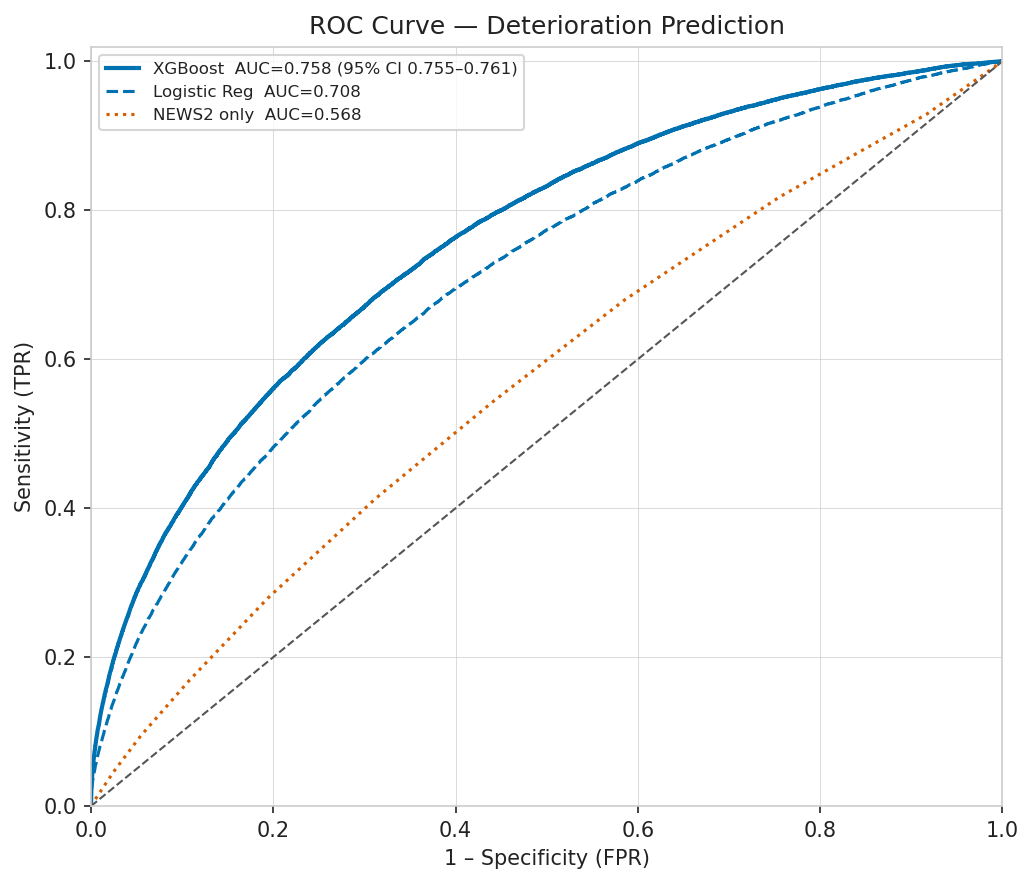
\includegraphics[width=\textwidth]{figures/roc_curve.png}
  \caption{\textbf{Supplementary Fig.~S1 — Receiver Operating Characteristic curves
    from model training.}
    ROC curves for XGBoost (blue) and logistic regression (orange), pooled from
    five-fold patient-stratified cross-validation. The diagonal dashed line
    represents a random classifier. AUROC values with 95\% bootstrap confidence
    intervals are annotated. The marked operating point corresponds to 90\%
    sensitivity at threshold = 0.31.}
  \label{fig:roc_supp}
\end{figure}

\begin{figure}[H]
  \centering
  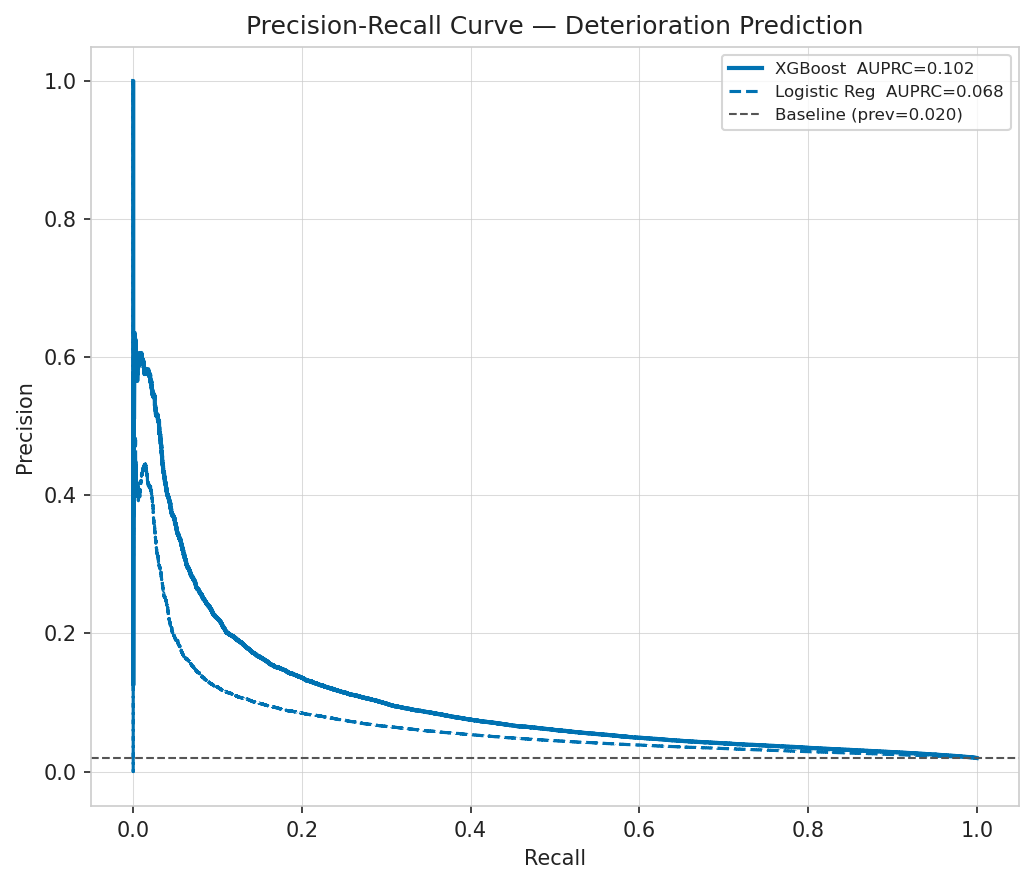
\includegraphics[width=\textwidth]{figures/pr_curve.png}
  \caption{\textbf{Supplementary Fig.~S2 — Precision-Recall curves.}
    Precision-recall curves for XGBoost (blue) and logistic regression (orange).
    The dashed horizontal line indicates the no-skill baseline equal to event
    prevalence (1.96\%). AUPRC values are annotated. The XGBoost model achieves
    AUPRC = 0.102, a 5.2-fold improvement over the prevalence baseline,
    indicating substantially better precision at clinically relevant recall
    thresholds.}
  \label{fig:pr_supp}
\end{figure}

\begin{figure}[H]
  \centering
  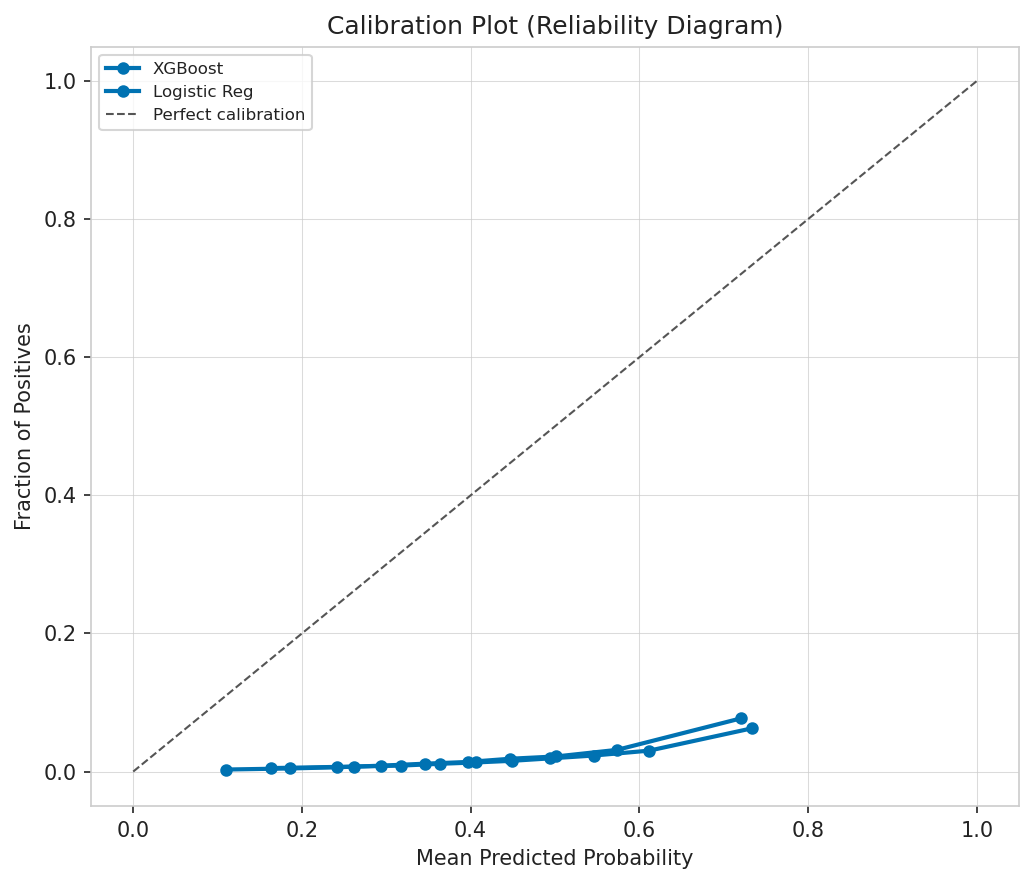
\includegraphics[width=\textwidth]{figures/calibration.png}
  \caption{\textbf{Supplementary Fig.~S3 — Calibration curves (reliability
    diagrams).}
    Reliability diagram comparing predicted probabilities (x-axis) against
    observed event fractions (y-axis) for XGBoost (blue) and logistic regression
    (orange). The diagonal dashed line represents perfect calibration. Brier
    scores are annotated. The XGBoost model (Brier score = 0.175) shows
    systematic overestimation above predicted probability 0.35, a known
    consequence of extreme class imbalance; predicted scores should be interpreted
    as relative risk rankings rather than absolute probabilities.}
  \label{fig:cal_supp}
\end{figure}

\begin{figure}[H]
  \centering
  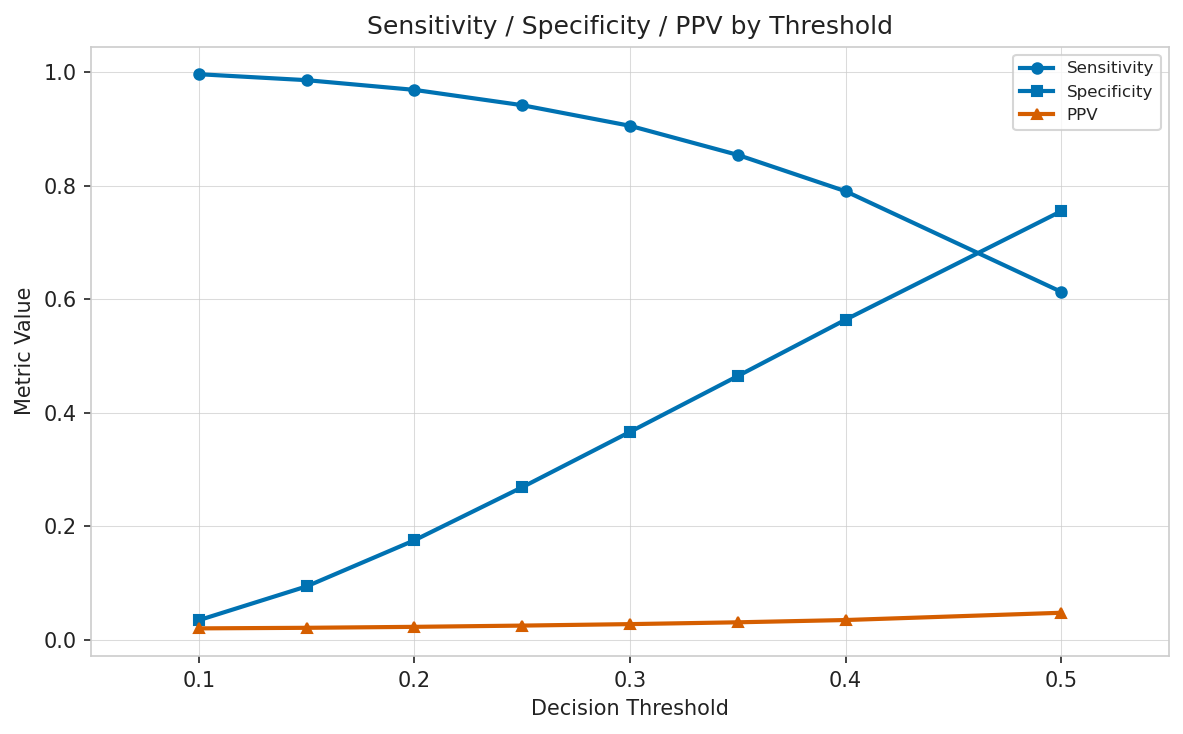
\includegraphics[width=\textwidth]{figures/threshold_analysis.png}
  \caption{\textbf{Supplementary Fig.~S4 — Threshold operating characteristics.}
    Sensitivity (blue), specificity (orange), PPV (green), and F1 score (red) as
    a function of decision threshold for the XGBoost model. The vertical dashed
    line marks the recommended threshold (0.31) corresponding to 90\% sensitivity.
    Institutions may adjust the threshold rightward to reduce alert burden at the
    cost of sensitivity, or leftward to maximise detection at the cost of
    increased false-positive alerts.}
  \label{fig:threshold_supp}
\end{figure}

%% ─────────────────────────────────────────────────────────────────────────────
%% REFERENCES
%% ─────────────────────────────────────────────────────────────────────────────
\clearpage
\bibliography{references}

\end{document}
